\section{Problem Setting}

Consider two indistinguishable particles in an infinite square well of length $L$. The Hilbert space of the system, $\mathcal{H}$, is constructed from the tensor product of the individual state-spaces, $\mathcal{H}_1$ and $\mathcal{H}_2$:
\begin{equation}
    \mathcal{H} = \mathcal{H}_1 \otimes \mathcal{H}_2
\end{equation}
The particles are confined to a configuration space where $(x_1, x_2)$ are within the well. The infinite well imposes Dirichlet boundary conditions, which means the wavefunction $\Psi(x_1, x_2)$ must be zero if either particle is at the boundary.

\section{The System Hamiltonian}

The Hamiltonian for the system is given by the sum of the kinetic energy and potential energy terms:
\begin{equation}
    \hat{H} = \hat{T} + \hat{V}_{\text{ext}} + \hat{V}_{\text{int}}
\end{equation}

\subsection{Kinetic and Potential Energy Terms}

The total kinetic energy, $\hat{T}$, is the sum of the individual kinetic energies for each particle. In operator form, these are:
\begin{align}
    \hat{T}_1 &= \frac{\hat{p}_1^2}{2m} \otimes I \\
    \hat{T}_2 &= I \otimes \frac{\hat{p}_2^2}{2m}
\end{align}
The external potential for an infinite square well is taken to be zero inside the well:
\begin{equation}
    \hat{V}_{\text{ext}}(x_i) = 0
\end{equation}
The particles have an inter-particle interaction modeled by a Dirac delta function, which is a contact interaction that occurs only when the particles are at the same position, $x_1 = x_2$:
\begin{equation}
    \hat{V}_{\text{int}}(x_1, x_2) = g\,\delta(x_1 - x_2)
\end{equation}
Combining these terms, the Hamiltonian in the position representation is:
\begin{equation}
    \hat{H}(x_1, x_2) = -\frac{\hbar^2}{2m}(\nabla_1^2 + \nabla_2^2) + g\,\delta(x_1 - x_2)
\end{equation}

\section{Symmetry and Indistinguishability}

Since we are working with two identical particles, we must consider the particle exchange operator $P_{12}$, defined by its action on the wavefunction:
\begin{equation}
    P_{12}\Psi(x_1, x_2) = \Psi(x_2, x_1)
\end{equation}
This operator commutes with the Hamiltonian, $[P_{12}, \hat{H}] = 0$. This is a crucial property, as it means that if an initial state has a specific exchange symmetry, that symmetry will be preserved for all time.
\begin{itemize}
    \item \textbf{Symmetric}: If $\Psi(x_1, x_2, 0) = \Psi(x_2, x_1, 0) \Rightarrow P_{12}\Psi(x_1, x_2, t) = \Psi(x_1, x_2, t)$.
    \item \textbf{Antisymmetric}: If $\Psi(x_1, x_2, 0) = -\Psi(x_2, x_1, 0) \Rightarrow P_{12}\Psi(x_1, x_2, t) = -\Psi(x_1, x_2, t)$.
\end{itemize}
Given the Spin-Statistics Theorem, one must distinguish between bosons (exchange-symmetric states) and fermions (exchange-antisymmetric states). In the present work, we restrict our attention exclusively to the fermionic case, leaving the analysis of bosonic systems aside.


We focus on the case of two indistinguishable fermions confined in a one-dimensional box. For such particles, the state vector must belong to the antisymmetric subspace of the total Hilbert space. A general antisymmetric two-particle state $|\psi_A\rangle$ can therefore be written as:
\begin{equation}
|\psi_A\rangle = \frac{1}{\sqrt{2}} \left( |\psi_1\rangle \otimes |\psi_2\rangle - |\psi_2\rangle \otimes |\psi_1\rangle \right).
\end{equation}

\section{The Schrödinger Equation in Position Representation}

The dynamics of the fermionic system are described by the time-dependent Schr"odinger equation. In the position representation, the equation reads:
\begin{equation}
i\hbar\frac{\partial}{\partial t}\Psi_A(x_1, x_2, t) = \left[ -\frac{\hbar^2}{2m}(\nabla_1^2 + \nabla_2^2) + g,\delta(x_1 - x_2) \right] \Psi_A(x_1, x_2, t).
\end{equation}

\section*{5. Separation of Variables and Ansatz}

We look for separable solutions in space and time as our first ansatz, of the form:
\begin{equation}
\Psi(x_1, x_2, t) = \Psi_{n,\kappa}(x_1, x_2),\phi_t(t).
\end{equation}

To construct an antisymmetric spatial function for fermions, we use two single-particle eigenfunctions, $\phi_n(x)$ and $\phi_\kappa(x)$, and combine them as follows:
\begin{equation}
\Psi_F(x_1, x_2, t) = \frac{1}{\sqrt{2}}\left[\phi_n(x_1)\phi_\kappa(x_2) - \phi_n(x_2)\phi_\kappa(x_1)\right]\phi_t(t),
\end{equation}
which correctly satisfies the antisymmetry condition required for fermionic states.
where the single-particle functions (our second ansatz) are given by:
\begin{equation}
    \phi_n(x_i) = \sqrt{\frac{2}{L}}\sin\left(\frac{n\pi x_i}{L}\right),
\end{equation}
and the temporal factor corresponds to the usual energy eigenstate exponential, a result of the separable form of the time-dependent Schrödinger equation:
\begin{equation}
    \phi_t(t) = e^{-iEt/\hbar}.
\end{equation}

Substituting both expressions into the fermionic ansatz, we obtain the complete wavefunction:
\begin{align}
    \Psi_F(x_1, x_2, t) = \sqrt{\frac{1}{2}}\left[\sqrt{\frac{2}{L}}\sin\left(\frac{n\pi x_1}{L}\right)\sqrt{\frac{2}{L}}\sin\left(\frac{\kappa\pi x_2}{L}\right)
    - \sqrt{\frac{2}{L}}\sin\left(\frac{\kappa\pi x_1}{L}\right)\sqrt{\frac{2}{L}}\sin\left(\frac{n\pi x_2}{L}\right)\right] e^{-iEt/\hbar}.
\end{align}

Simplifying the prefactors, the final normalized antisymmetric fermionic wavefunction becomes:
\begin{equation}
    \Psi_F(x_1, x_2, t) =
    \frac{1}{\sqrt{L^2}}
    \left[
    \sin\left(\frac{n\pi x_1}{L}\right)\sin\left(\frac{\kappa\pi x_2}{L}\right)
    - \sin\left(\frac{\kappa\pi x_1}{L}\right)\sin\left(\frac{n\pi x_2}{L}\right)
    \right]
    e^{-iEt/\hbar},
\end{equation}

\subsection*{4. Expectation Value of the Interaction for Fermions}

The expectation value of the interaction potential $V = g\,\delta(x_1 - x_2)$ in a fermionic state is:
\begin{equation}
    \langle \psi_F | V | \psi_F \rangle = g\int_{0}^{L}\int_{0}^{L} \psi_F^{*}(x_1, x_2)\,\psi_F(x_1, x_2)\,\delta(x_1 - x_2)\,dx_1\,dx_2.
\end{equation}

Because $\psi_F(x,x)=0$ for all $x$ in $[0,L]$, the integrand vanishes on the support of the delta distribution and therefore:
\begin{equation}
    \langle \psi_F | V | \psi_F \rangle = 0.
\end{equation}

\subsection*{5. Determination of the Energy}

Substituting the ansatz into the Schr\"odinger equation and separating space and time yields:
\begin{align}
    -\frac{\hbar^{2}}{2m}\left(\frac{\partial^{2}\Psi_{n,\kappa}}{\partial x_1^{2}} + \frac{\partial^{2}\Psi_{n,\kappa}}{\partial x_2^{2}}\right) &= E\,\Psi_{n,\kappa}, \\
    i\hbar \frac{1}{\phi_t}\frac{d\phi_t}{dt} &= E.
\end{align}

Thus the spatial energy eigenvalue reads:
\begin{equation}
    E = -\frac{\hbar^{2}}{2m}\frac{\left(\partial_{x_1}^{2}\Psi_{n,\kappa} + \partial_{x_2}^{2}\Psi_{n,\kappa}\right)}{\Psi_{n,\kappa}}.
\end{equation}

Using that for the single-particle eigenfunctions $\partial_{x_i}^{2}\phi_n(x_i) = -n^{2}\omega^{2}\phi_n(x_i)$ with $\omega = \pi/L$, one obtains:
\begin{equation}
    \partial_{x_1}^{2}\Psi_{n,\kappa} + \partial_{x_2}^{2}\Psi_{n,\kappa} = -\omega^{2}(n^{2} + \kappa^{2})\Psi_{n,\kappa}.
\end{equation}

Hence the energy associated with the two-particle antisymmetric state is:
\begin{equation}
    E = \frac{\hbar^{2}\omega^{2}}{2m}(n^{2} + \kappa^{2}) = \frac{\pi^{2}\hbar^{2}}{2mL^{2}}(n^{2} + \kappa^{2}).
\end{equation}

\subsection*{6. Final Form of the Wavefunction}

The complete fermionic wavefunction for the considered state is therefore:


\begin{equation}
    \Psi_F(x_1, x_2, t) = \frac{1}{\sqrt{2}}
    \left[
    \sin\left(\frac{n\pi x_1}{L}\right)\sin\left(\frac{\kappa\pi x_2}{L}\right)
    - \sin\left(\frac{\kappa\pi x_1}{L}\right)\sin\left(\frac{n\pi x_2}{L}\right)
    \right]
    e^{-iEt/\hbar},
\end{equation}
with $E$ given above.

\begin{figure}[h!]
    \centering
    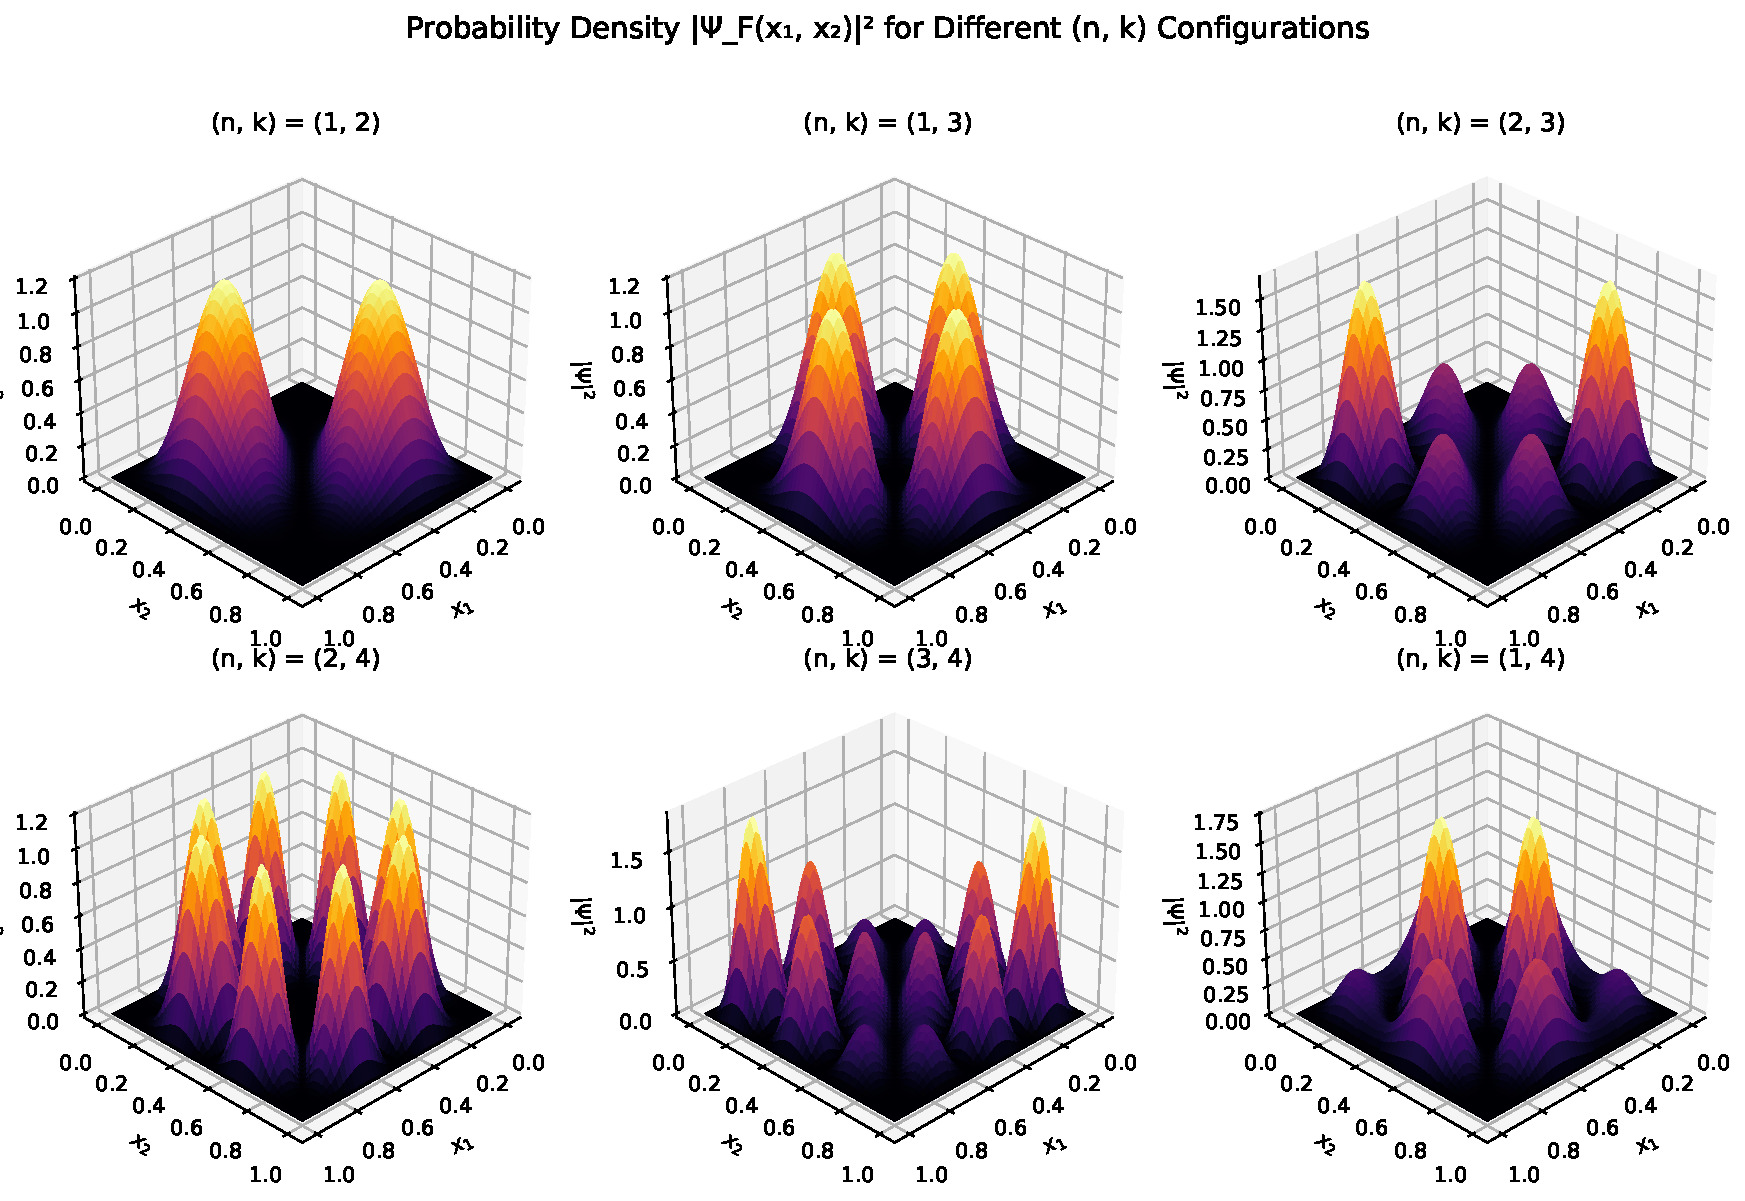
\includegraphics[width=0.9\textwidth]{ figures/fermions_3D_collage-1.pdf}
    \caption{Probability density $|\Psi_F(x_1, x_2)|^2$ for six antisymmetric two-fermion configurations
    $(n,\kappa) = (1,2), (1,3), (2,3), (2,4), (3,4), (1,4)$.
    The antisymmetric nature of the wavefunction enforces $\Psi_F(x_1 = x_2) = 0$, reflecting the Pauli exclusion principle.}
    \label{fig:fermion_3D_collage}
\end{figure}


\section{Remarks and Validity}

The derivation above is valid for the antisymmetric spatial sector (fermions) and for the idealized contact interaction represented by the delta potential. For bosonic states, the delta interaction generally yields nontrivial corrections to energy eigenvalues and must be treated using either regularization methods or matching conditions across the line $x_1=x_2$. The present fermionic ansatz trivially nullifies the delta contribution because of the vanishing of the wavefunction at coincidence points.
